\section{Evaluation}

In this section we will take a look at the performance of several different models using the aforementioned features. We will start off with some regression modeling and then move on to some classification modeling. Because of our small number of volunteers, we are unlikely to see great results; though we can at least get an idea of the performance of the models and features we use.

\subsection{Regression}

The first model we will consider a classic and a good starting point: the basic linear model. For these predictions, we split the data 80\% for training and 20\% for testing. The following performance values are the values calculated on the unseen test data. Using only the heart rate data, we found the model acheived extremely low performance, with an R$^2$ of 0.077 and root mean squared error (RMSE) of 0.036. Ideally, we want an R$^2$ value of 1.0 and an RMSE of 0.0. Adding in the skin temperature data boosted the R$^2$ up to 0.268 with 0.032 RMSE. Better, but still bad. Adding in the accelerometer data the values were 0.276 and 0.032, for R$^2$ and RMSE respectively. Even using all our preselected features, the linear model is just not a good fit.

So how does a more flexible model perform? We next trained a neural network model on the data. Training a neural network model is very expensive in terms of time, so we reduced our dataset to 8\% of the original. Of the remaining amount we used 70\% for training the model and 30\% for testing. The neural network itself had two hidden layers of five nodes each. This structure was determined experimentally while optimizing for training time and performance. In the input layer we used the heart rate, skin temperature, and accelerometer features. Figure \ref{fig:nn_all} plots the BAC predictions in of the neural network model on top of the actual values from the test set. The real values are jittered to give a sense of the density of the data, the prediction values in blue are not. Overall, the model achieved a much better R$^2$ value of 0.525, with RMSE of 0.026, than the linear regression model.

\begin{figure}
	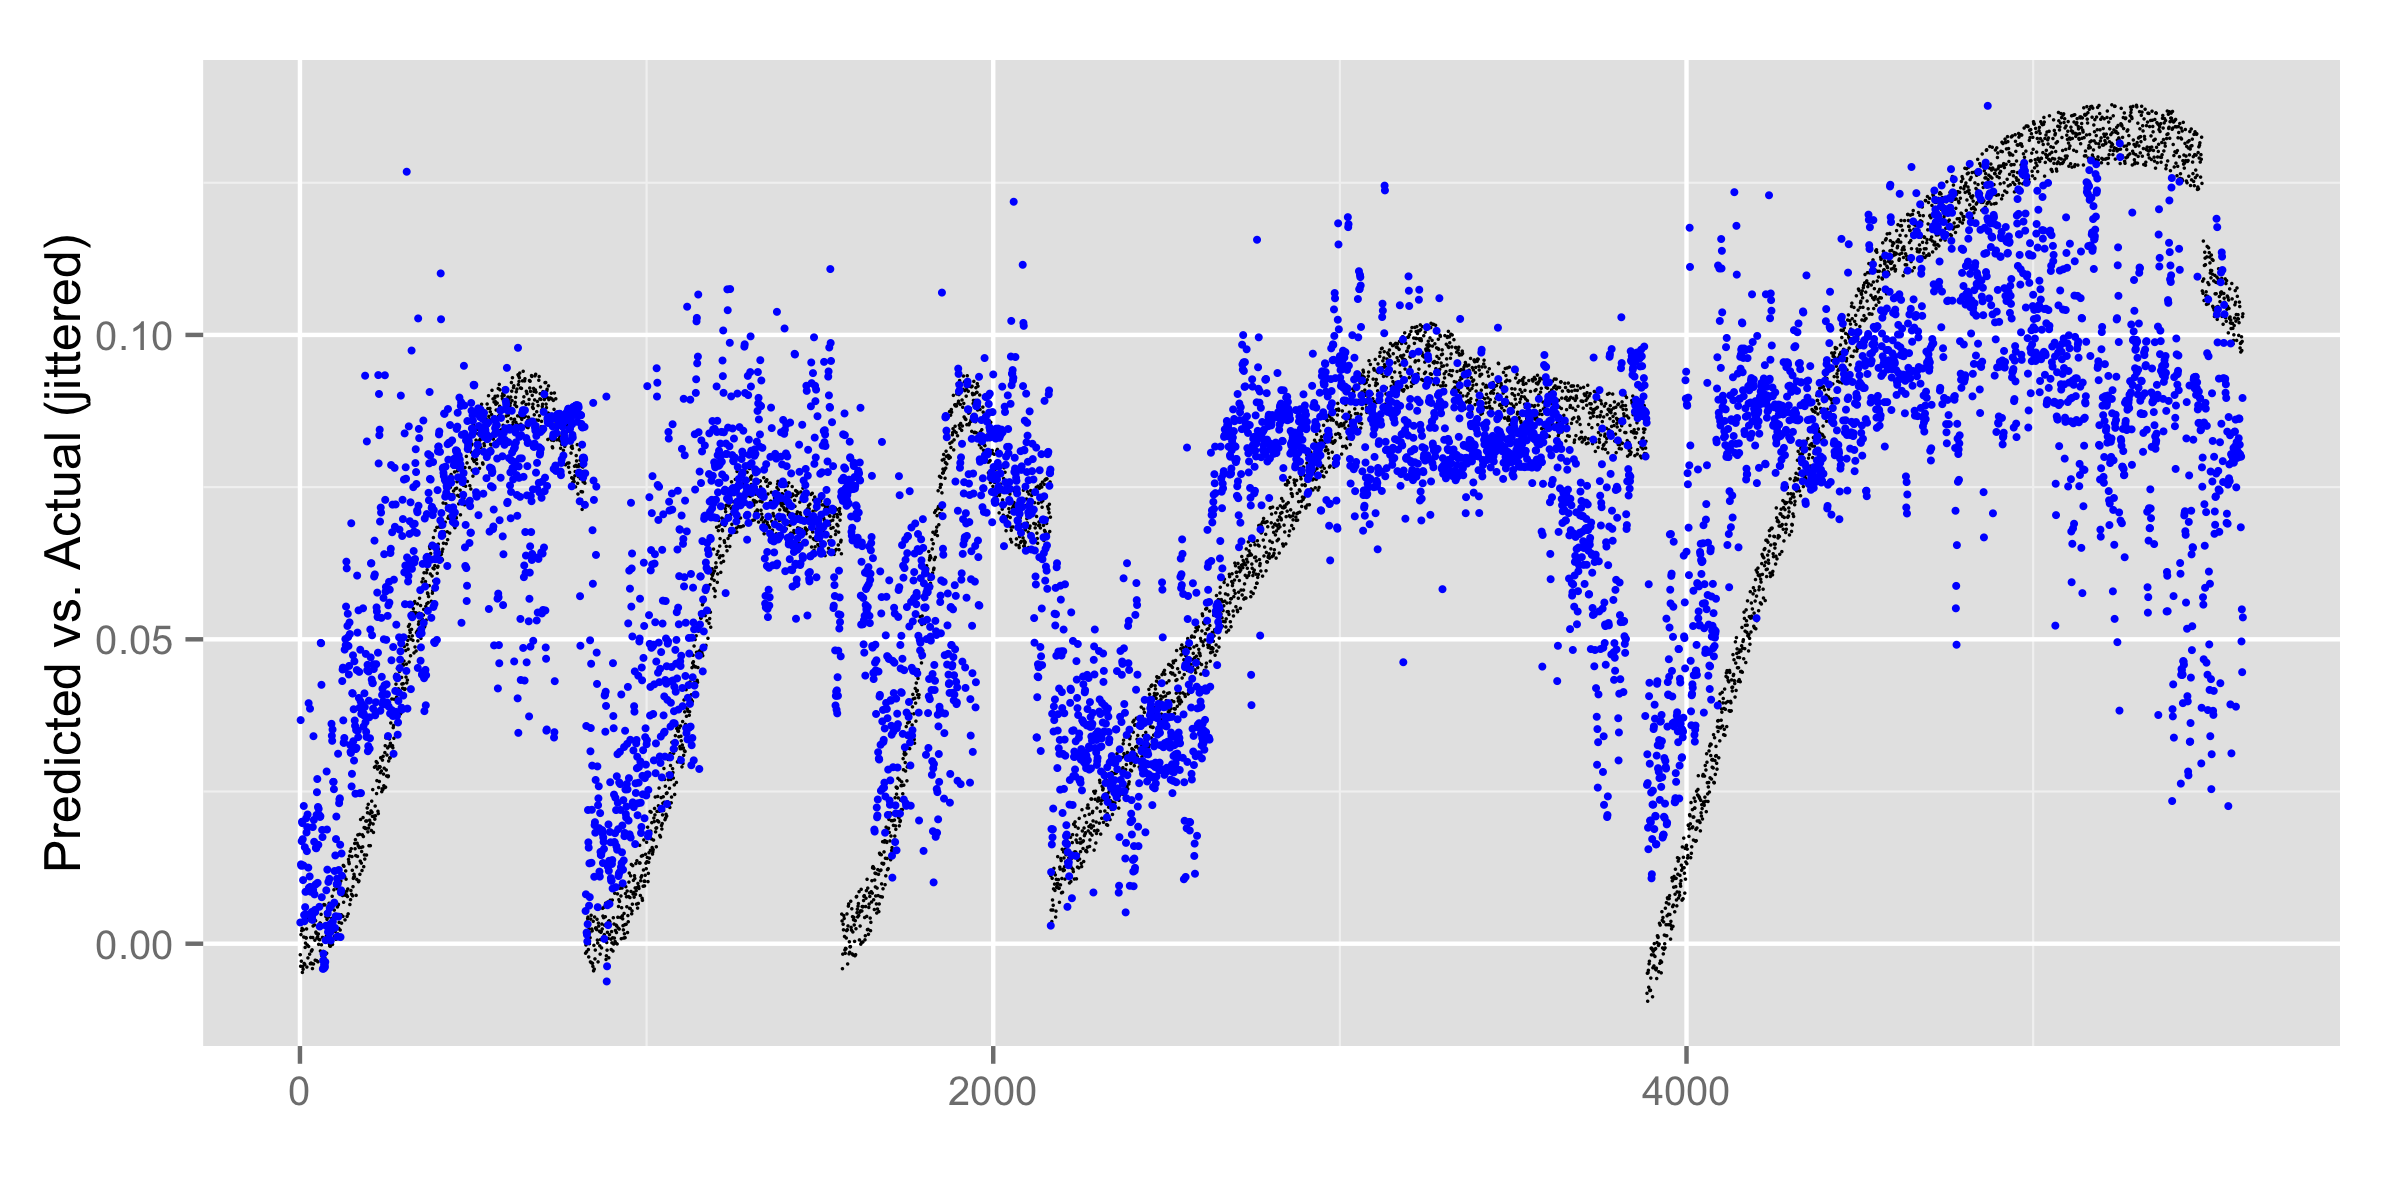
\includegraphics[width=1.0\textwidth]{../figs/nn_all}
	\caption{ANN predictions (blue) over actual BAC (black, jitterred) using test data.}
	\label{fig:nn_all}
\end{figure}

\subsection{Classification}

This problem might be better handled as a classification task. To do this we will first have to use a threshold to classify the existing BAC labels as \textit{DRUNK} or \textit{SOBER}. We want to warn a person if they are close to reaching the legal limit of 0.08 BAC. A good time to warn a user is at about 0.065 BAC. This splits the classes into 64\% is drunk, and 36\% sober.

The common logistic regression model will be the first to try for our classification task. To train the model, we split the data set by 80\% for training and 20\% for testing as we did for the linear regression model. We will also go ahead and use the full combination of heart, temperature, and accelerometer features. A logistic regression model outputs values from 0.0 to 1.0, so we need to determine where to best split this output into each class. In Figure \ref{fig:log_pred_density}, we show a plot of the predictions of the model on the test data, using the actual labels to distinguish the output. In this plot, we see that the best threshold value for the logistic model predictions is around 0.32; above that we classify \textit{SOBER} and below that \textit{DRUNK}. Using this split, we achieved a precision score of 0.852, recall of 0.730, and F1-score of 0.786.

\begin{figure}
	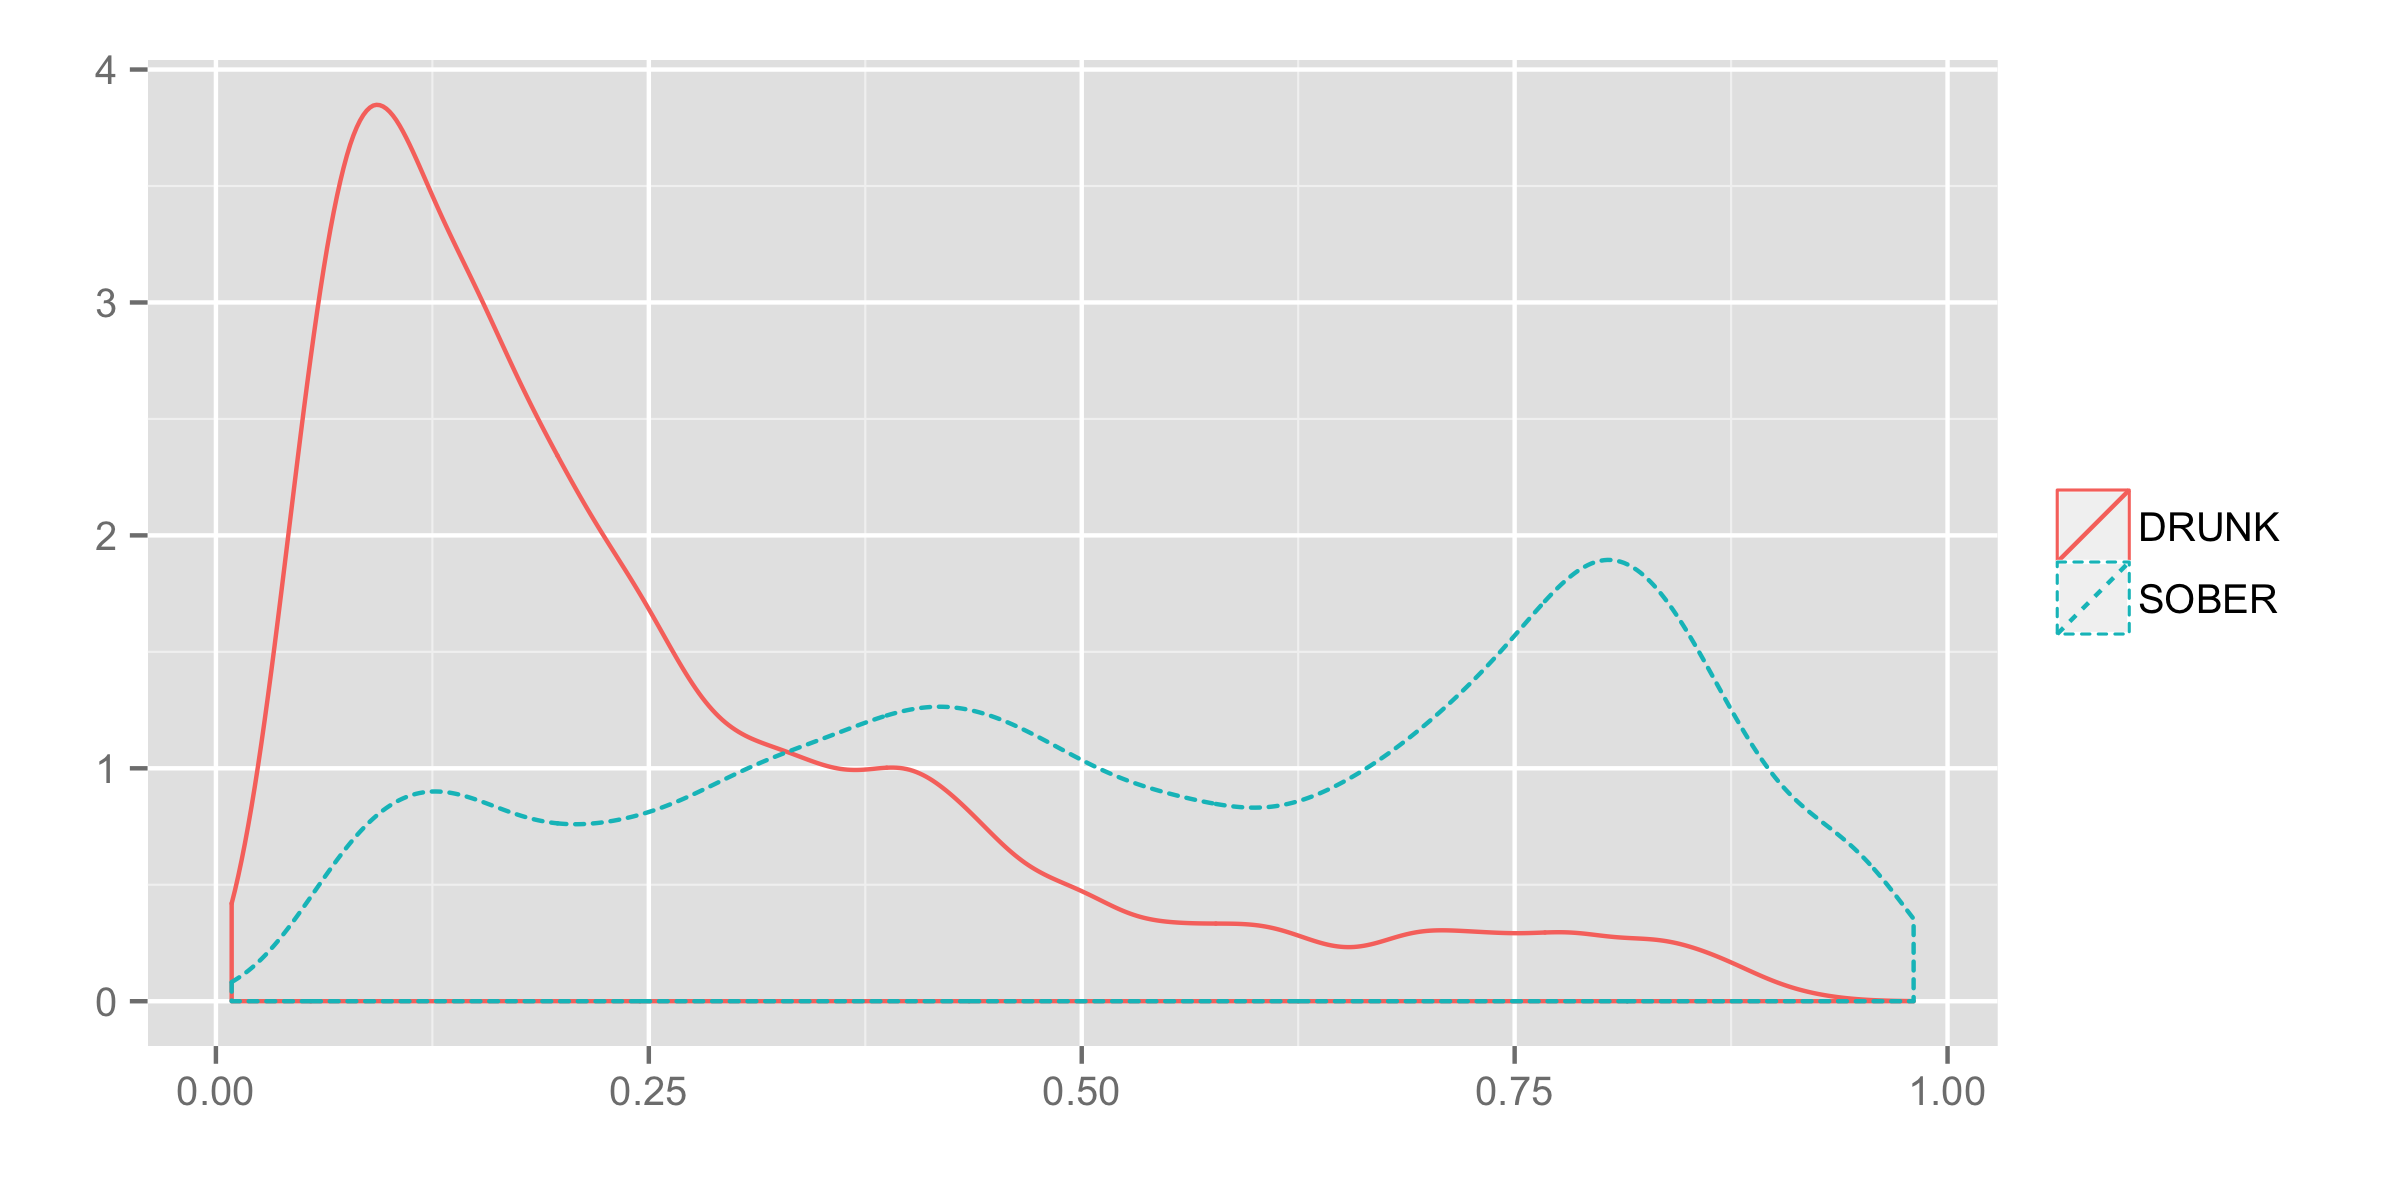
\includegraphics[width=1.0\textwidth]{../figs/log_pred_density}
	\caption{Logistic regression output frequency with actual labels.}
	\label{fig:log_pred_density}
\end{figure}

The final model we will consider is the SVM using the Gaussian Radial Basis Function (RBF) kernel. This time we first sampled 50\% of the data and then split this into 80\% for training and 20\% for testing. The initial reduction is performed because the SVM is very time-consuming to train, a bit faster than the ANN. On our 0.065-BAC-thresholded data, we found the SVM acheived great performance with a precision of 0.887, recall of 0.931, and overall F1-score of 0.909 on the test data. Ideally, we would not want to warn our users that they are drunk when they are not actually drunk, so we want to try and optimize the model to be as precise as possible. By modifying the error weighting to train against false positive errors, the SVM model achieved a precision of 0.974, with recall of 0.732, and F1-score of 0.836. Our recall dropped for a higher precision, which is a well-known tradeoff for this kind of tuning, but this is fine. We can set a threshold on our smartphone warning system that if at least a recall fraction of the samples from our smartwatch are classified as \textit{DRUNK}, then there is a precision chance that the user is actually at 0.065 BAC.